\documentclass{article}
\usepackage{amsfonts, amsthm, amsmath, amssymb, mathtools, ulem, mathrsfs, physics, esint, siunitx, tikz-cd}
\usepackage{pdfpages, fullpage, color, microtype, cancel, textcomp, markdown, hyperref, graphicx}
\usepackage{enumitem}
\graphicspath{{./images/}}
\usepackage[english]{babel}
\usepackage[autostyle, english=american]{csquotes}
\MakeOuterQuote{"}
\usepackage{xparse}
\usepackage{tikz}
\usepackage{algorithm}% http://ctan.org/pkg/algorithm
\usepackage{algpseudocode}% http://ctan.org/pkg/algorithmicx

% fonts
\def\mbb#1{\mathbb{#1}}
\def\mfk#1{\mathfrak{#1}}
\def\mbf#1{\mathbf{#1}}
\def\tbf#1{\textbf{#1}}

% common bold letters
\def\bP{\mbb{P}}
\def\bC{\mbb{C}}
\def\bH{\mbb{H}}
\def\bI{\mbb{I}}
\def\bR{\mbb{R}}
\def\bQ{\mbb{Q}}
\def\bZ{\mbb{Z}}
\def\bN{\mbb{N}}

% brackets
\newcommand{\br}[1]{\left(#1\right)}
\newcommand{\sbr}[1]{\left[#1\right]}
\newcommand{\brc}[1]{\left\{#1\right\}}
\newcommand{\lbr}[1]{\left\langle#1\right\rangle}

% matrices
\newcommand{\m}[2][b]{\begin{#1matrix}#2\end{#1matrix}}
\newcommand{\arr}[3][\sbr]{#1{\begin{array}{#2}#3\end{array}}}

% misc
\NewDocumentCommand{\app}{O{x} O{\infty}}{\xrightarrow{#1\to#2}}
\newcommand{\sse}{\subseteq}
\renewcommand{\ss}{\subset}
\newcommand{\vn}{\varnothing}
\newcommand{\e}{\epsilon}
\newcommand{\vp}{\varphi}
\renewcommand{\th}{\theta}
\newcommand{\inv}{^{-1}}
\newcommand{\imp}{\implies}
\newcommand{\impleft}{\reflectbox{$\implies$}}
\renewcommand{\ip}[2]{\lbr{#1,#2}}
\renewcommand{\bar}{\overline}
\DeclareMathOperator{\cis}{cis}
\DeclareMathOperator{\Arg}{Arg}
\renewcommand{\d}{\partial}
\renewcommand{\O}{\Omega}
\newcommand{\G}{\Gamma}
\newcommand{\g}{\gamma}
\newcommand{\p}{\rho}

% title
\title{Scientific Computing Final Exam}
\author{Ryan Chen}
%\date{\today}
\setlength{\parindent}{0pt}


\begin{document}
	
\maketitle



\begin{enumerate}
	
	
	
\item 

\begin{enumerate}
	
	
	\item Solution for $\mu=100$ on the left and $\mu=1000$ on the right.
	\begin{center}
		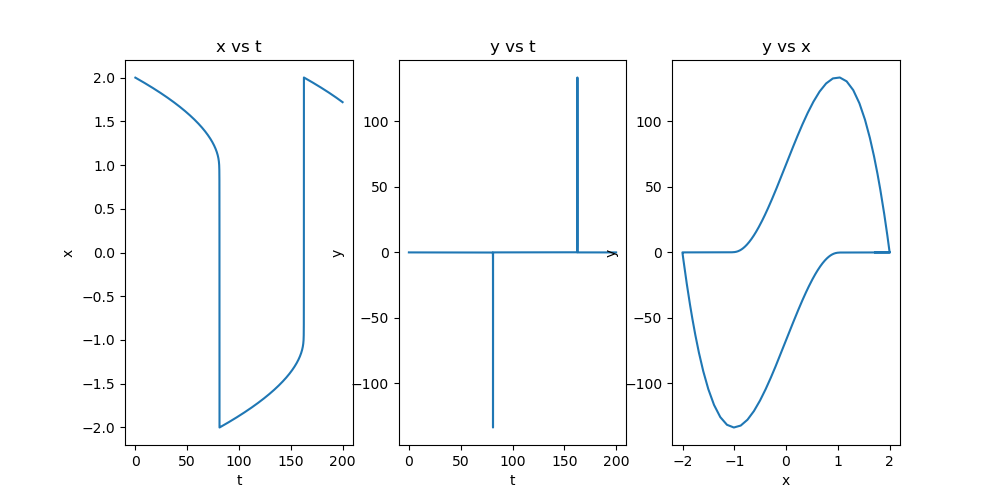
\includegraphics[scale=.2]{final 1 mu = 100}
		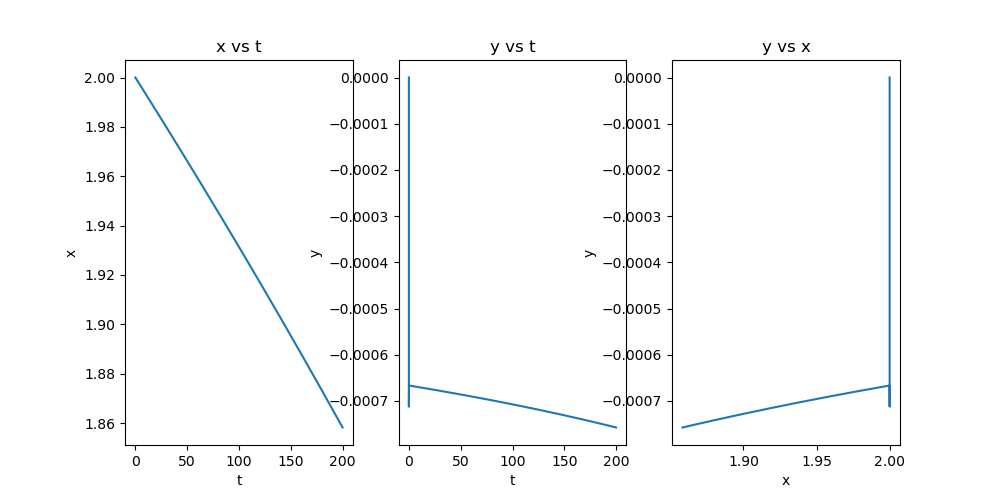
\includegraphics[scale=.2]{final 1 mu = 1000}
	\end{center}

	
	\item From the Butcher array, $\hat b=\m{1-\g\\\g}$ and $c=\m{\g\\1}$. Pick $b:=\m{1\\0}$. Then the method using $b$ is order 1 since $b_1+b_2=1$ but not order 2 since $b\cdot c=\g\ne\frac12$. The error estimate is
	\[e := h\sum_{q=1}^2(b-\hat b)_qk_q
	= h(\g k_1-\g k_2)
	= h\g(k_1-k_2)
	\imp \norm{e} = h\g\norm{k_1-k_2}\]
	
	The following adaptive time step algorithm multiplies or divides the time step by 2 to get close to the largest time step satisfying the step acceptance criterion.
	\begin{algorithmic}
			\State err $\gets$ h*gamma*norm(k1-k2)
			\State tol $\gets$ atol + rtol*norm([x,y])
			\If{err $<$ tol}
				\While{err $<$ tol}
					\State h $\gets$ 2*h
					\State compute k1 and k2 using h
					\State err $\gets$ h*gamma*norm(k1-k2)
				\EndWhile
			\EndIf
			\If{err $>$ tol}
				\While{err $>$ tol}
					\State h $\gets$ 0.5*h
					\State compute k1 and k2 using h
					\State err $\gets$ h*gamma*norm(k1-k2)
				\EndWhile
			\EndIf
	\end{algorithmic}
	
	CPU time of 409s.
	\begin{center}
		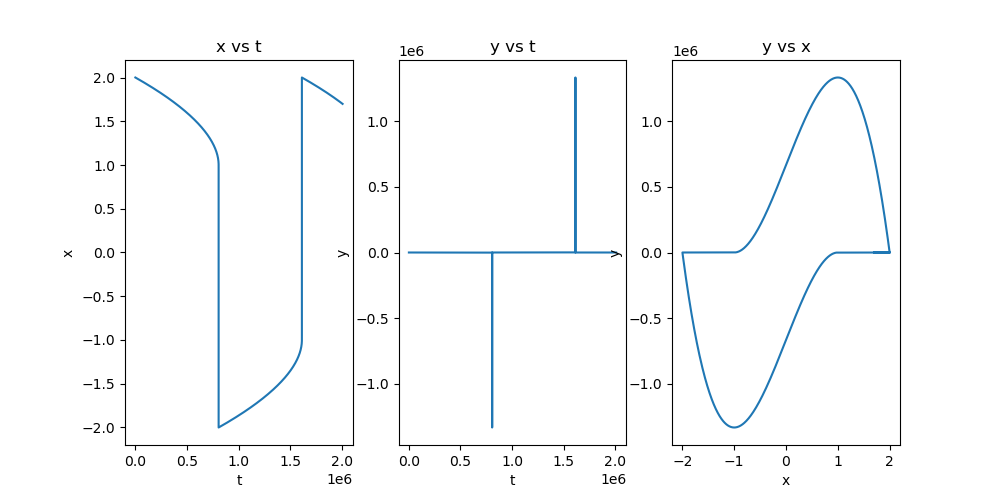
\includegraphics[scale=.6]{final 1 mu = 1000000}
	\end{center}
	
\end{enumerate}



\item

\begin{enumerate}
	
	
	\item As a preliminary, recall a "generalized" divergence theorem: for all scalars $\vp\in C^1(\O,\bR)$ and vectors $F\in C^1(\O,\bR^2)$,
	\[\int_\O\grad\vp\cdot Fdx = -\int_O\div Fdx + \int_{\d\O}\vp F\cdot nds\]
	Let $A(x,y):=e^{-\beta V(x,y)}M(x,y)$. Pick $u_D\in C^2(\bR^2)$ such that $u_D=0$ on $\d A$, $u_D=1$ on $\d B$, and $u_D=0$ outside some neighborhood of $\d B$ disjoint from $\G_N$ (an explicit formula for $u_D$ is given later). We obtain a BVP for $v:=u-u_D$,
	\[\div(A\grad v) = -\div(A\grad u_D),
	\quad v=0 \text{ on } \G_D:=\d A\cup\d B,
	\quad \pdv{v}{n}=0 \text{ on } \G_N\]
	Now fix $w\in C^1(\O)$ such that $w=0$ on $\G_D$, multiply the PDE for $v$ and integrate over $\O$.
	\[\int_O w\div(A\grad v)dx = -\int_O w\div(A\grad u_D)dx\]
	This equation, along with the generalized divergence theorem for $\vp:=w$ and $F:=A\grad v$, gives
	\[\int_\O A\grad w\cdot\grad vdx = \int_\O w\div(A\grad u_D)dx + \int_{\G_D} wA\pdv{v}{n}ds + \int_{\G_N} wA\pdv{v}{n}ds\]
	On the RHS, the second term vanishes since $w=0$ on $\G_D$, and the third term vanishes since $\pdv{v}{n}=0$ on $\G_N$. The generalized divergence theorem for $\vp:=w$ and $F:=A\grad u_D$ gives
	\[\int_\O A\grad w\cdot\grad u_Ddx = -\int_\O w\div(A\grad u_D)dx + \int_{\G_D} wA\pdv{u_D}{n}ds + \int_{\G_N} wA\pdv{u_D}{n}ds\]
	On the RHS, the second term vanishes since $w=0$ on $\G_D$, and the third term vanishes since $u_D=0$ on $\G_N$. Combining the last two equations gives
	\[\int_\O A\grad w\cdot\grad vdx = -\int_\O A\grad w\cdot\grad u_Ddx\]
	This is the integral equation formulation for all solutions to the BVP for $v$ and for all $w\in C^1(\O)$.
	
	The standard mollifier on $\bR^2$ is
	\[\eta(x) :=
	\begin{cases}
		C\exp(\frac{1}{\norm{x}^2-1}), & \norm{x} < 1 \\
		0, & \norm{x} \ge 1
	\end{cases}\]
	with $C$ such that $\int_{\bR^2}\eta dx=1$. The family of mollifiers for $\e>0$ is
	\[\eta_\e(x) := \frac{1}{\e^2}\eta\br{\frac x\e}\]
	Note that the support of $\eta_\e$ is the open ball with center $(0,0)$ and radius $\e$. Pick $u_D$ to be a mollifier which equals 1 on $\d B$ and vanishes at points more than 0.1 away from $\d B$.
	\[u_D(x) := \frac{1}{\eta_{0.3}(0.2,0)}\eta_{0.3}(x-(0.5,0.1))\]
	
	
\end{enumerate}



\item

\begin{enumerate}
	
	
	\item Rewrite the PDE as
	\[\p_t + [f(\p)]_x = 0,
	\quad f(\p) := \p v(\p) = \p - \p^3\]
	Characteristics are given by
	\[x(t) = f'(\p_0(x_0))t + x_0,
	\quad f'(\p) = 1 - 3\p^2\]
	They are plotted below.
	\begin{center}
		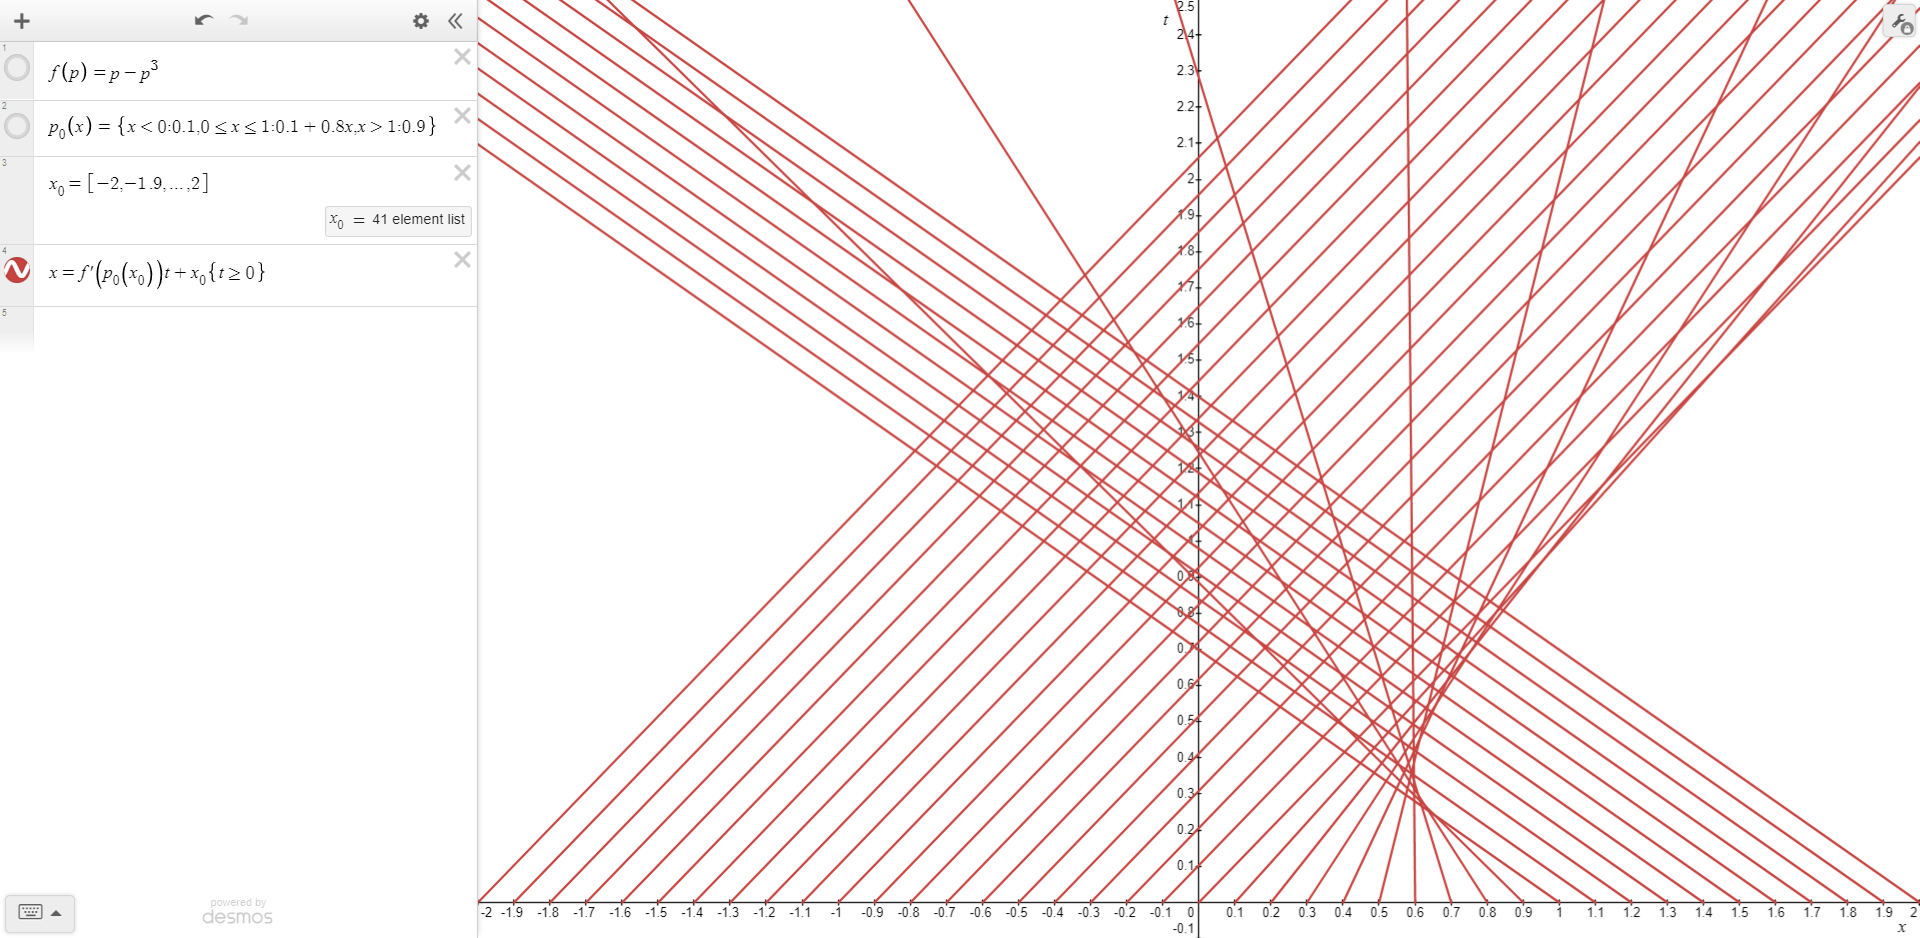
\includegraphics[scale=.3]{final 3a}
	\end{center}


	\item The breaking time, when the first shock occurs, is
	\[T_b = -\sbr{\min_zf''(\p_0(z))\p_0'(z)}\inv \approx 0.231\]
	The equation for $\p_0$ gives $\p_L=0.1$ and $\p_R=0.9$, so the eventual shock speed is
	\[s = \frac{f(\p_L)-f(\p_R)}{\p_L-\p_R} = 0.09\]
	
	
\end{enumerate}



\end{enumerate}
	
	
\end{document}